% ===================================================================
% 1. Introduction
% ===================================================================
\section{Introduction}
\label{sec:intro}

The ability to perceive the exact 6D pose — comprising a 3D translation vector $\bt \in \R^3$ and a 3$\times$3 rotation matrix $\bR \in \SO$ — of an object is a fundamental prerequisite for advanced robotic interactions in unstructured environments. While 2D object detection has seen tremendous advancements with the advent of Convolutional Neural Networks (CNNs), lifting these predictions into the 3D space remains challenging due to the loss of depth information during the camera projection process.

The standard LineMod protocol~\cite{hinterstoisser2012model} makes this problem harder in a specific and instructive way: only $\sim$15\% of the real frames of each object sequence are available for training, and the remaining 85\% form the test set. State-of-the-art methods cope with this data scarcity either by generating tens of thousands of additional synthetic training images per object~\cite{he2020pvn3d, he2021ffb6d}, or by architecturally grounding the prediction in the observed 3D points through dense per-pixel fusion~\cite{wang2019densefusion}. In this work we investigate a third, considerably cheaper route: keeping a lightweight global-fusion architecture and real-only training data, and changing only the \emph{formulation} of the regression target.

Our pipeline is structured in three consecutive phases:

\begin{enumerate}
    \item \textbf{2D Object Detection.} We establish a robust 2D detection framework using YOLO11n~\cite{ultralytics2024yolo11} to extract precise Regions of Interest (RoI), evaluated through the stringent mAP@50-95 metric.

    \item \textbf{RGB-only Baseline.} We develop an RGB-only baseline utilizing a ResNet-50 backbone equipped with a dual regression head to predict both the translation vector and the rotation quaternion, exposing the structural depth ambiguity of monocular estimation.

    \item \textbf{RGB-D Global Fusion with anchored regression.} We introduce a lightweight RGB-D Global Fusion architecture that concatenates globally pooled RGB, depth, and camera-metadata features. Its translation head does not regress an absolute position: it predicts a residual with respect to a 3D \emph{anchor} back-projected from the depth observed inside the detected bounding box. Rotations use the 6D continuous representation of Zhou~\etal~\cite{zhou2019continuity}.
\end{enumerate}

We evaluate on the official LineMod split, training on 2{,}016 real images and testing on 13{,}407, with no synthetic data. Our main contributions are as follows:

\begin{itemize}
    \item An \textbf{anchored residual formulation} of the translation target for global RGB-D fusion: with architecture, data, and training recipe held fixed, it lifts ADD(-S) accuracy from 6.8\% (direct absolute regression) to 95.1\% in a fully end-to-end evaluation with predicted detections.
    \item A controlled \textbf{ablation over geometry input representations} (raw metric depth, anchor-normalized depth, per-pixel XYZ maps) showing that the anchoring of the target — not the richness of the input encoding — is the decisive factor.
    \item A \textbf{memorization analysis} of the result: retrieval- and oracle-nearest-neighbor baselines bound any pose-copying strategy at 7.1\% on this protocol, and accuracy remains stable up to $12^\circ$ of viewpoint novelty, ruling out memorization as an explanation.
    \item The resulting system outperforms the per-pixel variant of DenseFusion (86.2\%)~\cite{wang2019densefusion} under the same protocol and data regime, while remaining a $\sim$36M-parameter architecture with no per-point processing and no refinement stage.
\end{itemize}

Qualitative results of the anchored model on cluttered LineMod scenes are shown in Figure~\ref{fig:teaser}: across diverse object geometries the predicted 3D bounding boxes (red) align tightly with the ground truth (green), from detections produced by the retrained YOLO11n (blue).

\begin{figure*}[t]
    \centering
    \begin{subfigure}[t]{0.245\textwidth}
        \centering
        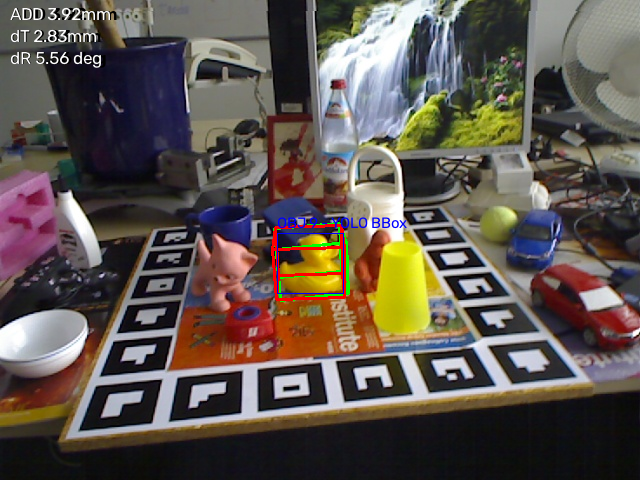
\includegraphics[width=\linewidth]{figure/v2/qualitative/obj09_add3.92mm.png}
        \caption{duck --- ADD 3.9\,mm}
    \end{subfigure}\hfill
    \begin{subfigure}[t]{0.245\textwidth}
        \centering
        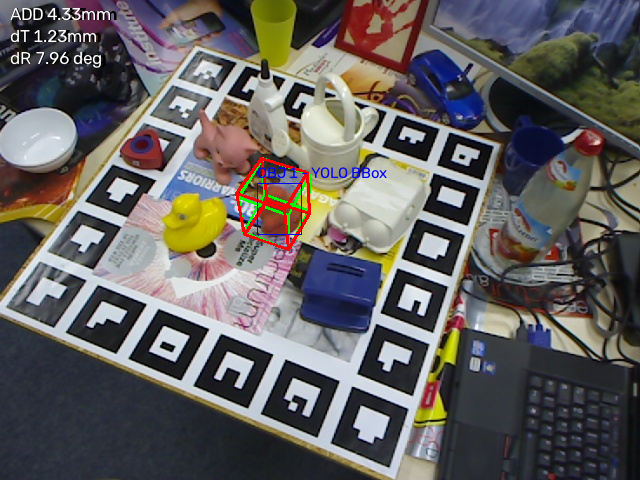
\includegraphics[width=\linewidth]{figure/v2/qualitative/obj01_add4.33mm.png}
        \caption{ape --- ADD 4.3\,mm}
    \end{subfigure}\hfill
    \begin{subfigure}[t]{0.245\textwidth}
        \centering
        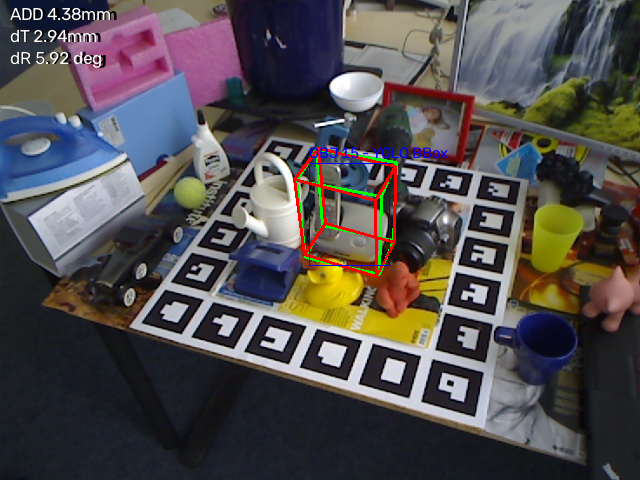
\includegraphics[width=\linewidth]{figure/v2/qualitative/obj15_add4.38mm.png}
        \caption{phone --- ADD 4.4\,mm}
    \end{subfigure}\hfill
    \begin{subfigure}[t]{0.245\textwidth}
        \centering
        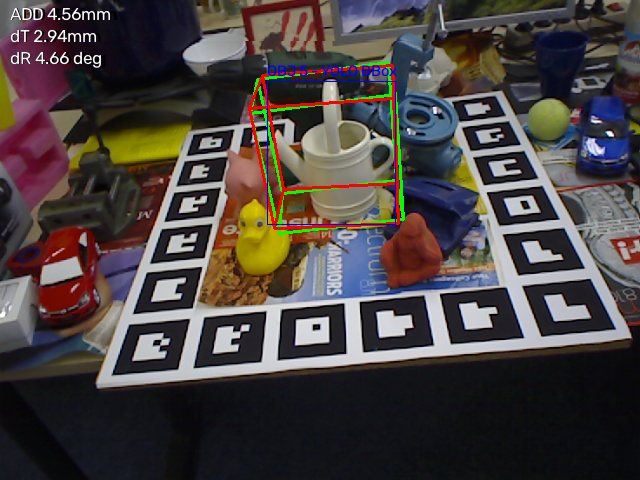
\includegraphics[width=\linewidth]{figure/v2/qualitative/obj05_add4.56mm.png}
        \caption{can --- ADD 4.6\,mm}
    \end{subfigure}
    \caption{Qualitative end-to-end results of the anchored \texttt{norm} model on the official LineMod test set. Green: ground-truth 3D box; red: prediction; blue: YOLO11n detection used for crop, metadata, and anchor.}
    \label{fig:teaser}
\end{figure*}
